\documentclass[11pt,a4paper]{article}
\usepackage[top=3cm, bottom=3cm, left=2.5cm, right=2.2cm]{geometry} %geometry of page
\usepackage[hidelinks]{hyperref} %reference links
\usepackage{fancyhdr} %header and footer control
\usepackage{minted} %source code syntax highlighting
\usepackage{qrcode} %qrcode links
\usepackage{graphicx} %images
\usepackage{tikz} %diagrams
\usetikzlibrary{calc}

\linespread{1.3}
\emergencystretch 3em

% Set Header and Footer
\fancyhead{}
\fancyhead[L]{\textbf{Lab 4: Hall effect sensor}}
\fancyhead[R]{d.s.brennan@sheffield.ac.uk}
\fancyfoot{}
\fancyfoot[L]{\thepage}
\fancyfoot[R]{MAC 233 Arduino Labs, School of MAC, University of Sheffield}

% Create Document
\begin{document}
\pagestyle{fancy}

\section*{Prerequisites}
This lab doesn't require any code from previous labs; however, it does expect you to have completed these, as common code repeated from previous labs will not be explained in detail again here. Out of your Arduino pack, you will need: 1 Arduino, 1 A3144 hall effect sensor, 1 LED, 1 $10K\Omega$ resistor, 1 $220\Omega$ resistor, and 5 jumper cables.

\section*{Objectives}
The objective of today's lab is to learn how to use an interrupt to record a value of a sensor whose value is changed via an external event: \url{https://docs.arduino.cc/language-reference/en/functions/external-interrupts/attachInterrupt/}.\\

\noindent
This worksheet will take you through the steps of how to connect a hall effect sensor to your Arduino, monitor when the value of the sensor has changed, and provide visual feedback to an end user of when the value has changed.

\section*{Hall effect sensors}
In short, a hall effect sensor allows you to detect the presence of a magnet --- the value given by the sensor changes when a magnet is near to it. This type of sensor has many applications, but most importantly for us, is it provides the facility to detect movement and ultimately how quick that movement was.\\

\begin{figure}[ht]
    \begin{center}
        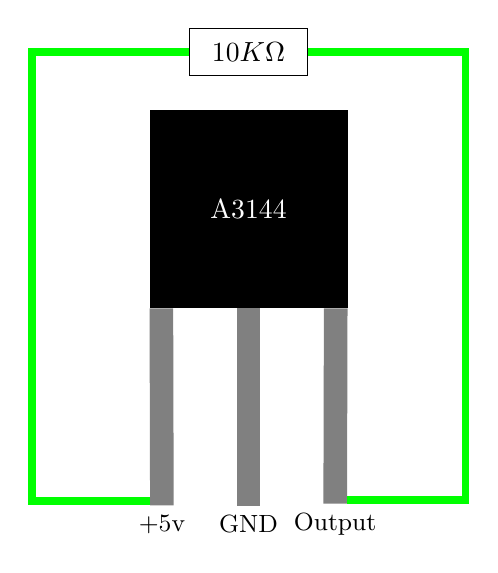
\begin{tikzpicture}[
            sensor/.style={fill=black, draw=black, text=white, minimum size=2.5cm},
            resistor/.style={fill=none, draw=black, text=black, minimum height=.6cm, minimum width=1.5cm},
            pin/.style={draw=gray, line width=3mm},
            wire/.style={line width=1mm},
            label/.style={draw=none, text=black},
        ]
            %% components
            \node[resistor] at (0, 2) (resistor) {$10K\Omega$};
            \node[sensor] at (0, 0) (hall-effect){A3144};
            \node[label] at (-1.1, -4) (positive) {\small +5v};
            \node[label] at (0, -4) (ground) {\small GND};
            \node[label] at (1.1, -4) (output) {\small Output};
            %% pin
            \draw[pin] ($(hall-effect.south west) + (0.15, 0)$) -- (positive);
            \draw[pin] (hall-effect.south) -- (ground);
            \draw[pin] ($(hall-effect.south east) - (0.15, 0)$) -- (output);
            %% connection
            \draw[wire, draw=green] let \p1 = ($(positive.north) + (-0.155, 0.05)$), \p2 = ($(\p1) - (1.5, 0)$), \p3 = (resistor.west) in (\p1) -- (\p2) -- (\x2, \y3) -- (\p3);
            \draw[wire, draw=green] let \p1 = ($(output.north) + (0.155, 0.05)$), \p2 = ($(\p1) + (1.5, 0)$), \p3 = (resistor.east) in (\p1) -- (\p2) -- (\x2, \y3) -- (\p3);

        \end{tikzpicture}
    \end{center}
    \caption{The wiring diagram of our hall effect sensor. The sensor has two bases on a trapezium. This wiring diagram is with the short base facing towards you.}
    \label{fig:hall-effect-sensor}
\end{figure}

\noindent
The particular hall effect sensor you have has three legs: a \textit{power} leg, a \textit{ground} leg, and a \textit{digital output} leg. The sensor is shaped like a trapezium. With the short base of the trapezium facing towards you (as depicted in Figure \ref{fig:hall-effect-sensor}) and the legs facing south, the sensor is wired into the Arduino as follows: Arduino +5V\textrightarrow left leg, Arduino GND\textrightarrow middle leg, and Arduino Pin D2\textrightarrow right leg.\\

\section*{Interrupts}
The purpose of today's lab, is to gain experience of when and how to use an \textit{interrupt} in an Arduino. In previous labs, we have changed the value of an externally connected device using the command \textit{digitalWrite}. You can read the value of a sensor using the command \textit{digitalRead}; however, this method is not always appropriate when you consider when within the event timeline, the value of the sensor may change.\\

\noindent
If we consider how an Arduino works in context of an event timeline. The Arduino runs the code within the `setup' function, then runs the code in the `loop' function continuously until it is turned off. If we were to put as the first line of the `loop' function \textit{digitalRead(PIN)}, we could capture the value of pin at the beginning of the loop. The Arduino would then execute the rest of the code within the `loop' function, then start the `loop' again, at which point we would then capture the current value of the pin again.\\

\noindent
This design pattern works well in a system that is designed to monitor the gradual change of a value over a period of time --- say capturing the temperature outside every five minutes over a twenty-four-hour period; however, this design pattern fails in a scenario where the sensor value could have changed between the two instances of the \textit{digitalRead} logic. In this scenario you need a way of interrupting the Arduino to pause whatever it is doing, run the required code needed to record a value change, and then continue with its previous operations; an \textit{interrupt}.\\

\noindent
Because being able to interrupt the `loop' function is a special case, there may be restrictions --- depending on your Arduino --- as to which pins this feature is enabled on. In the case of the Nano family of Arduino's, this is digital pins: 2 \& 3 (\url{https://www.arduino.cc/reference/cs/language/functions/external-interrupts/attachinterrupt/}).\\

\section{Creating the circuit}
\label{sec:circuit}
There are two circuits needed for this worksheet, the first is for the hall effect sensor (HES), and the second is for the visual display LED.\\
\noindent
\textbf{HES circuit}: Arduino +5V\textrightarrow\hspace{0.1em}HES left leg, Arduino GND\textrightarrow\hspace{0.1em}HES middle leg, Arduino Pin D2\textrightarrow\hspace{0.1em}HES right leg. HES left\textrightarrow \hspace{0.1em}$10K\Omega$ resistor\textrightarrow\hspace{0.1em}HES right legs.\\
\noindent
\textbf{LED circuit}: Arduino Pin D4\textrightarrow $220\Omega$ resistor\textrightarrow LED\textrightarrow Arduino GND.\\


\section{System Functionality}
\label{sec:functionality}
The basis of this system is that we have an LED and a hall effect sensor --- say placed near the crank of a bike --- connected to our Arduino as described in Section \ref{sec:circuit}. We set up the LED as we did in Lab 2 (but on a different pin) and then attach an interrupt to the pin connected with the hall effect sensor. Every time a magnet passes past the field of the hall effect sensor --- say a magnet on the crank arm of a bike --- the associated interrupt code is called, and it records the time in milliseconds of that event. Within the `loop' function, we can then calculate if the last time the interrupt happened, is  within a 500-millisecond window of the current time. If true, we can turn on the LED, if false, we turn off the LED.\\

\noindent
The first thing we need to do is create a blank sketch, this is done by opening Arduino IDE, going to `File'\textrightarrow `Examples'\textrightarrow `01.Basics'\textrightarrow `BareMinimum'. Once this has opened, we can now start to code up the system.\\

\noindent
The code within this section should all be placed within the global scope. Like our previous labs, the first piece of code included is defining the external pins and our constants. In our scenario, this is declaring the `$CRANK\_PIN $' for our hall effect sensor, and then our `$CRANK\_ACTIVITY\_LED\_PIN$' for our visual feedback as to when the hall effect sensor has been triggered. The last part of code is defining the 500-millisecond window in which we will activate the LED:\\
\vspace{-1.75em}
\inputminted{arduino}{./src/1-define.txt}
\vspace{.75em}

\noindent
Next, we need two global variables: `$current\_loop\_time$' to store a consistent execution time in milliseconds across the `loop' function, and a `$crank\_interrupt\_current\_time$' to store the time in milliseconds of the last recorded interrupt:\\
\vspace{-1.75em}
\inputminted{arduino}{./src/2-system-variables.txt}
\vspace{.75em}

\noindent
\textit{Note:} The reason we need to store a consistent time across the `loop' function is that the `loop' function may take 20 milliseconds to execute a full iteration of itself. If you request the current time (the \textit{millis()} function) at the beginning of the code, compared to the end of the code, you would get a different value; therefore, to ensure you have a consistent `current time' across an iteration of the `loop' function, you store the value at the beginning of the iteration and then use that referenced value throughout the function.\\

\section{Setup function}
The code required for the setup function can be thought of as three steps: 1 - enable debugging tools, 2 - initialise global values, 3 - set the pins to the correct modes and attach the interrupt.

\subsection{Enable debugging tools}
Enable the debugging through the serial: (\textit{hint:} see section 3.1 of Lab 3):\\
\vspace{-1.75em}
\inputminted{arduino}{./src/3-setup-debug.txt}
\vspace{.75em}

\subsection{Initialise global variables}
Both of the global system variables (`$current\_loop\_time$' \& `$crank\_interrupt\_current\_time$') have been created but have not been initialised; they exist, but they haven't been given any initial value. As both of these variables are of the data type \textit{unsigned long} a logical value for initialisation would be zero (the first possible valid value):\\
\vspace{-1.75em}
\inputminted{arduino}{./src/4-setup-defaults.txt}
\vspace{.75em}

\subsection{Pins}
The last thing to do within the `setup' function, is to set up the pins. The LED pin needs to be set to mode \textit{OUTPUT} and then to ensure the LED isn't already on, write to the LED a \textit{LOW} value to turn it off. Next, the hall effect sensor pin needs to be set to mode \textit{INPUT} and an interrupt needs to be added to the pin. In code terms, the interrupt is a separate function that is only called when the interrupt is triggered. In our code, this is a function called `$crankInterrupt$' that we define in the next section of the worksheet. All we are doing in the `setup' function, is referencing the `$crankInterrupt$' function, we do not create the function itself.\\

\noindent
There are several options when you attach the interrupt to define when the interrupt function is called. In our case we are using the \textit{FALLING} mode (\url{https://docs.arduino.cc/language-reference/en/functions/external-interrupts/attachInterrupt/#parameters}) as our hall effect sensors report a \textit{HIGH} value when no magnet is present, then the value then drops when a magnet is present:\\
\vspace{-1.75em}
\inputminted{arduino}{./src/5-setup-io.txt}
\vspace{.75em}

\section{Interrupt}
As discussed above, we need a new function that appears in the global scope --- like the `setup' \& `loop' function --- which can be called by the interrupt attached to the hall effect sensor pin. All this method does is record the current time in milliseconds to the `$crank\_interrupt\_current\_time$' variable. As an interrupt is stopping everything else running on an Arduino, you try to keep the code inside the interrupt to the bare minimum required: in our case, this is simply recording the time. All the intensive computational logic is done within the `loop' function --- determining if the LED should be on and thus turning on or off the LED.\\
\vspace{-1.75em}
\inputminted{arduino}{./src/6-interrupt.txt}
\vspace{.75em}

\section{Loop function}
The main logic of the loop can be divided into two steps: 1 - calculate if the last occurrence of the interrupt is within the 500-millisecond window, 2 - wait.

\subsection{Calculate window}
The first part for calculating the window is storing into the `$current\_loop\_time$' variable the current time in milliseconds. Next, you calculate if the current time and the last occurrence of the interrupt are within the 500-millisecond window. If true, you turn on the LED with the standard \textit{digitalWrite} method. We also then display a debug message so that if the LED isn't working, we can still see that the logic in the Arduino is working correctly. If the window has passed, we turn off the LED:\\
\vspace{-1.75em}
\inputminted{arduino}{./src/7-loop-led.txt}
\vspace{.75em}

\subsection{Wait}
The final logic within the `loop' function is to wait 50 milliseconds before the next iteration of the `loop' function:\\
\vspace{-1.75em}
\inputminted{arduino}{./src/8-loop-sleep.txt}
\vspace{.75em}

\section*{Try it out on your Arduino}
You now should be able to compile your sketch (`Sketch'\textrightarrow `Verify/Compile') and then upload to your Arduino (`Sketch'\textrightarrow `Upload'). You should now be able to pass the magnet across a side of the hall effect sensor, and every time you do, it should light up the LED. \textit{Note:} the hall effect sensors are directional, so if the LED isn't lighting up, turn over the magnet and try again.

\pagebreak
\section*{Help}
If you are having issue compiling the project or don't understand where each section goes, you can see a complete version of the sketch with additional source code comments at \url{https://github.com/dsbrennan/mac-233-arduino-labs/blob/main/lab-4-hall-effect-sensor/lab-4-hall-effect-sensor.ino}.

\begin{center}
    \qrcode[hyperlink, height=4cm]{https://github.com/dsbrennan/mac-233-arduino-labs/blob/main/lab-4-hall-effect-sensor/lab-4-hall-effect-sensor.ino}
\end{center}

\vspace{2em}

\noindent
Additionally, if you are wondering how to wire up the circuit required for this lab on the breadboard, the electronic wiring diagram is below.

\begin{center}
    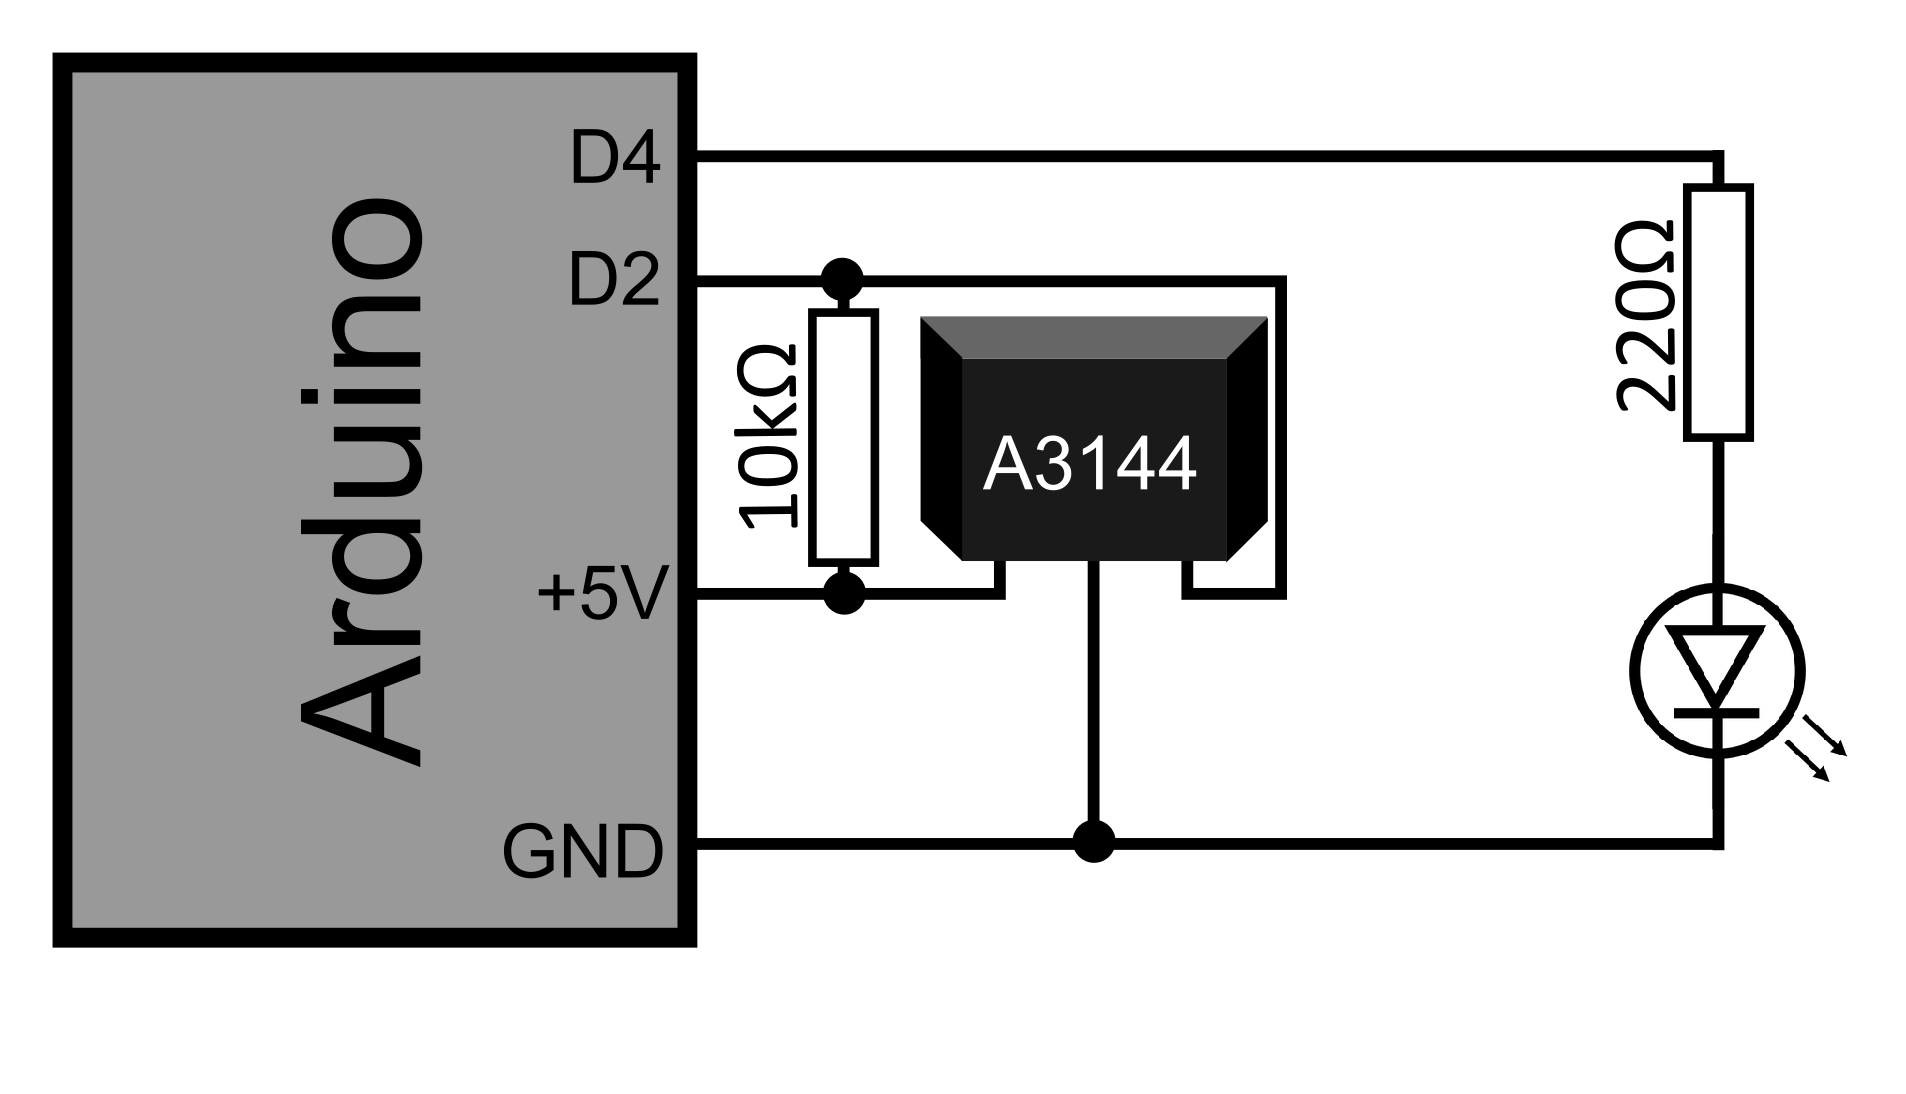
\includegraphics[width=.6\textwidth]{./images/wiring-diagram.png}
\end{center}

\end{document}